\chapter{Projeto/Proposta de Solução}
	\label{ch:proposta}

Os conceitos revisados até este momento serão utilizados para a criação de uma proposta de solução computacional para a equipe baja Velociraptor. Revisando, a equipe tem como principal problema não conseguir obter informações que interessam a cada setor de projeto do veículo de maneira \textbf{intuitiva, simplificada, modular e com armazenamento.} Estes três conceitos são detalhados no Quadro \ref{tab:cenario} a seguir:     

\begin{table}[!htb]
	\centering
		\caption{Conceitos do cenário estudado}
		\label{tab:cenario}
	\begin{tabular}{|l|l|l|}
		\hline
		\rowcolor[HTML]{9B9B9B} 
		{\color[HTML]{000000} Conceito} & {\color[HTML]{000000} Descrição}                                                                                                                                 \\ \hline
		Intuitiva                       & \begin{tabular}[c]{@{}l@{}}Demostração dos dados com \\ gráficos e valores absolutos\end{tabular}                                                                \\ \hline
		Simplificada                    & \begin{tabular}[c]{@{}l@{}}Um sistema para aquisição \\ para todos os dados dos sensores\\ reunindo as informações de \\ todos os setores do veículo\end{tabular} \\ \hline
		Modular                    & \begin{tabular}[c]{@{}l@{}}Preparado para expansão e\\  atualização com novas \\tecnologias\end{tabular} \\ \hline
		Armazenamento                   & \begin{tabular}[c]{@{}l@{}}Armazena os dados retirados \\ dos sensores para análises \\ futuras\end{tabular}                                                     \\ \hline
	\end{tabular}
		\caption*{Fonte: Autor.}
\end{table}

\section{Objetivos}
\label{sec:objetivos}
Os objetivos que devem nortear o trabalho a fim de sanar os problemas levantados podem ser subdivididos em objetivo principal, que é a meta final do trabalho, e objetivos específicos, que servem para medir a assertividade das medidas tomadas no curso do trabalho.

\subsection{Objetivo Geral}

Produzir um sistema que forneça a equipe informações que irão ajudar aos setores de projeto do veículo como suspensão dianteira, suspensão traseira, freio, transmissão e eletrônica em testes de bancada, bem como fornecer dados de uso geral da equipe como média do consumo de gasolina em prova para análises posteriores. 

O sistema é dividido em duas frentes: a parte de \textbf{aquisição} dos dados, feito junto ao SCOB com base nos dados recebidos via sensores revisados na seção \ref{sec:sensores}, esta parte já existe atualmente no baja Velociraptor, porém ela deve ser atualizada para acompanhar os avanços do novo \textit{software}; a parte de \textbf{tratamento} dos dados é o foco deste trabalho, nesta parte os dados serão transmitidos por um módulo de transmissão de dados sem fio ZigBee e lidos por um \textit{software} que permite visualização de gráficos e mostra de valores absolutos de maior importância. A Figura \ref{fig:esquemageral} possui dois diagramas, o diagrama da Figura \ref{fig:esquemageral}\subref{fig:geralatual} traz um esquema geral que atualmente é utilizado pelo Velociraptor no seu projeto, já a Figura \ref{fig:esquemageral}\subref{fig:geralproposto} traz um esquema geral proposto para este trabalho de conclusão de curso, desde a aquisição dos dados pelos SCOBs até o tratamento dos dados nos boxes com o \textit{software}. Em ambas as figuras os balões em azul indicam os sensores, os balões em laranja indicam \textit{hardware} de controle e balões em verde indicam \textit{software}, os balões com texto em negrito indicam modificação/criação de um sistema.         

%\begin{figure}[!htb]
%	\centering
%		\caption{Diagrama com o esquema geral proposto do sistema.}
%		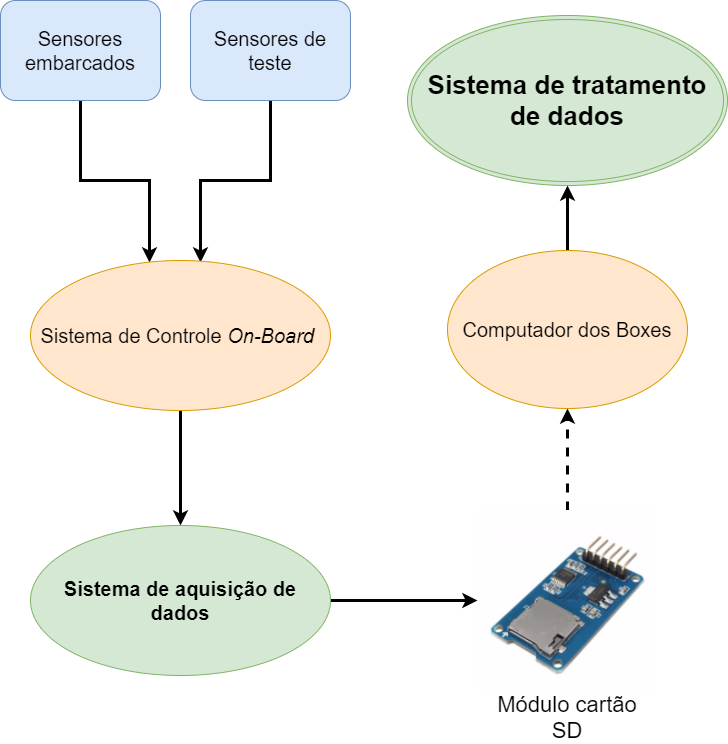
\includegraphics[scale=0.3]{geral.png} 
%		\caption*{Fonte: Autor.}
%		\label{fig:geral}
%\end{figure} 

\begin{figure}[!htb]
	\center
	\caption{Diagrama com o esquema geral do sistema atual e o esquema geral do sistema proposto.}
	\subfigure[Fonte: Autor][Esquema atual. Fonte:Autor]{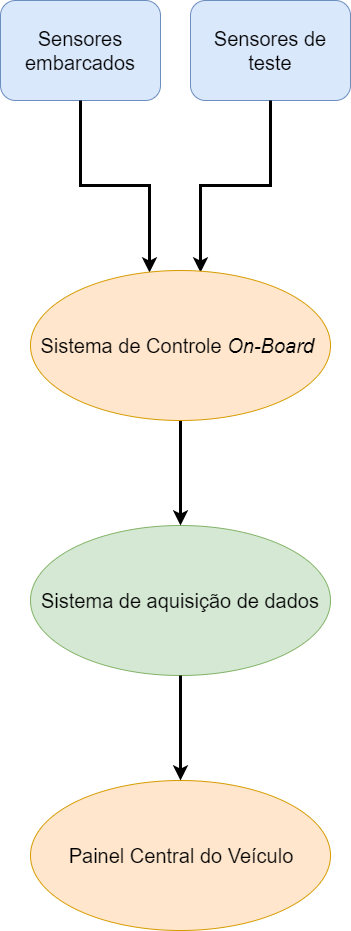
\includegraphics[scale=0.3]{geralatual}\label{fig:geralatual}}
	\qquad
	\subfigure[Fonte: Autor][Esquema proposto. Fonte:Autor]{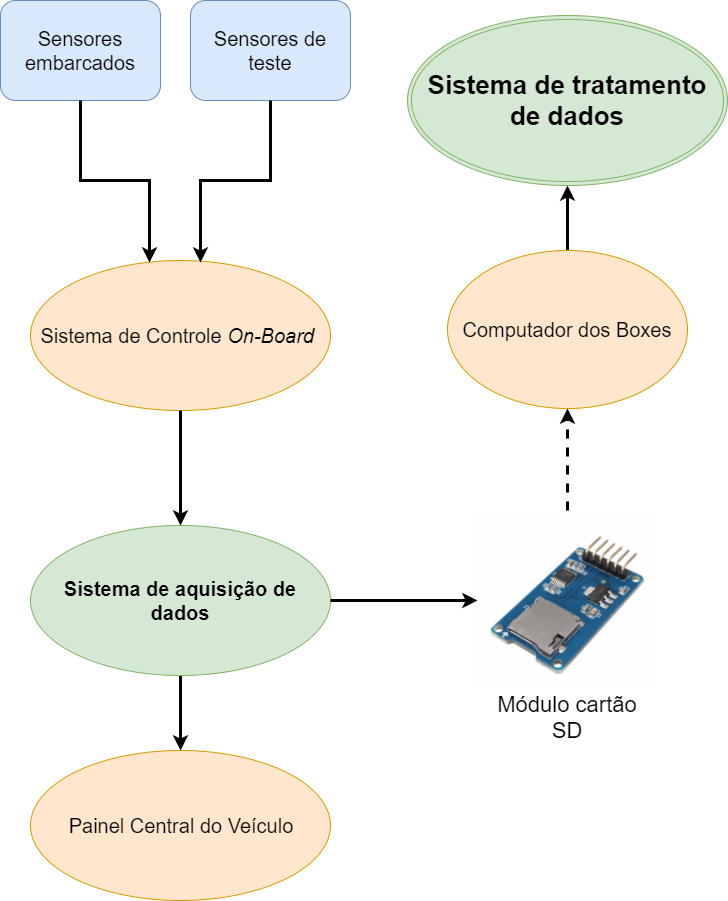
\includegraphics[scale=0.3]{geralproposto}\label{fig:geralproposto}}
	\label{fig:esquemageral}
\end{figure}


\subsection{Objetivos Específicos} 

\begin{itemize}[label={-}]
	\item O sistema deve ser independente em relação ao meio em que os dados são transportados do SCOB para os boxes, desta forma em atualizações futuras o método atual de transferência de dados pode ser substituído;
	\item O \textit{software} deve ser independente de sistema operacional;
	\item O \textit{software} deve possuir informações específicas para cada área da engenharia automobilística;
	\item O \textit{software} deve ser construído de forma a facilitar a manutenção evolutiva, preparado para chegada de novos sensores;
	\item Deve se instaurar uma cultura de utilização de plataformas de versionamento para facilitar manutenções adaptativas e manutenções corretivas.
\end{itemize}

Os objetivos específicos devem nortear a produção deste sistema. Atingindo as metas propostas se espera que o objetivo geral do projeto seja alcançado, trazendo essas informações do veículo para a equipe presente nos boxes.

\subsection{Mudanças de escopo}
O projeto teve uma mudança importante que deve ser citada. No início do processo de desenvolvimento do sistema, algumas reuniões com a equipe Velociraptor levaram a mudança do escopo antigo de trabalho, com utilização do módulo SD, para uma abordagem que utiliza de telemetria com módulos ZigBee. Esta mudança foi feita para acompanhar o projeto anual do sub-sistema de eletrônica embarcada sendo que esta mudança era uma meta inicial do projeto para trabalhos futuros. A mudança foi realizada tendo em vista a melhor abrangia do escopo, fazendo com que o resultado final seja mais consistente no quesito de entrega de resultados reais. Estas mudanças de escopo são também discutidas na Seção \ref{sec:hardwareutilizado}.